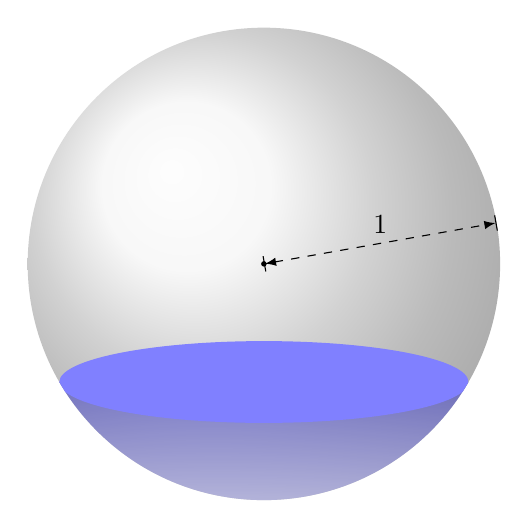
\begin{tikzpicture}[>=latex]
    \def\r{3}
    \def\H{1.5}
    \begin{scope}
    \clip 
    ({\r*cos(-90)},{\r*sin(-90)}) arc [start angle=-90,end
    angle=270,radius=\r];
    \shade[ball color=gray!15,opacity=0.5] (0,0) circle (\r);
    \shade[top color=blue!50!gray,bottom color=blue!20!white,opacity=0.6] 
 ({-\r},{-1.1*\r}) rectangle ++({2*\r},{0.1*\r+\H});
    \fill[blue!50] (0,{-\r+\H}) circle [x radius={sqrt(\r^2-(\r-\H)^2)},
    y radius={0.2*sqrt(\r^2-(\r-\H)^2)}];
    \end{scope}
    \fill[fill=black] (0,0) circle (1pt);
    \draw[dashed,|<->|] (0,0 ) -- node[above]{$1$} (10:\r);
    %\draw[|<->|] (4,{-\r}) --
    %    node[fill=white,font=\footnotesize,inner ysep=2pt,inner xsep=0]{$h$}
    %    (4,{-\r+\H});
\end{tikzpicture}

\begin{tikzpicture}%[font = \sansmath]
  \coordinate (O) at (0,0);

  % ball background color
  \shade[ball color = blue, opacity = 0.5] (0,0) circle [radius = 2cm];

  % cone
  \begin{scope}
    \def\rx{0.71}% horizontal radius of the ellipse
    \def\ry{0.15}% vertical radius of the ellipse
    \def\z{0.725}% distance from center of ellipse to origin

    \path [name path = ellipse]    (0,\z) ellipse ({\rx} and {\ry});
    \path [name path = horizontal] (-\rx,\z-\ry*\ry/\z)
                                -- (\rx,\z-\ry*\ry/\z);
    \path [name intersections = {of = ellipse and horizontal}];

    % radius to base of cone in ball
    \draw[fill = gray!50, gray!50] (intersection-1) -- (0,0)
      -- (intersection-2) -- cycle;
    % base of cone in ball
    \draw[fill = gray!30, densely dashed] (0,\z) ellipse ({\rx} and {\ry});
  \end{scope}

  % label of cone
  \draw (0.25,0.4) -- (0.9,0.1) node at (1.05,0.0) {$q$};

  % ball
  \draw (O) circle [radius=2cm];
  % label of ball center point
  \filldraw (O) circle (1pt) node[below] {$P$};

  % radius
  \draw[densely dashed] (O) to [edge label = $r$] (-1.33,1.33);
  \draw[densely dashed] (O) -- (1.33,1.33);

  % cut of ball surface
  \draw[red] (-1.35,1.47) arc [start angle = 140, end angle = 40,
    x radius = 17.6mm, y radius = 14.75mm];
  \draw[red, densely dashed] (-1.36,1.46) arc [start angle = 170, end angle = 10,
    x radius = 13.8mm, y radius = 3.6mm];
  \draw[red] (-1.29,1.52) arc [start angle=-200, end angle = 20,
    x radius = 13.75mm, y radius = 3.15mm];

  % label of cut of ball surface
  \draw (-1.2,2.2) -- (-0.53,1.83) node at (-1.37,2.37) {$A$};
\end{tikzpicture}